\documentclass[twoside,9pt]{report}
\usepackage[a5paper]{geometry}
\usepackage{newpxmath}
%\usepackage{libertine} \usepackage[libertine]{newtxmath}
%\usepackage{kpfonts}
\usepackage{graphicx}
\usepackage{listings}
\usepackage[T1]{fontenc}
\usepackage{imakeidx}
\usepackage{marginnote}
\usepackage[table]{xcolor}
\usepackage{caption}
\usepackage{etoc}
\lstset{
  showstringspaces=false,
  language=tcl,
  frame=lines,
  aboveskip=\bigskipamount,
  belowskip=\bigskipamount,
  numbers=left,
  numberstyle=\tiny,
  firstnumber=last,
  basicstyle=\small\ttfamily,
}
%\renewcommand{\thesection}{\arabic{section}}
\title{Into the Interpreter\\with ConsTcl}
\author{Peter Lewerin}
\date{\today}
\makeatletter
\def\@makechapterhead#1{%
  \vspace*{50\p@}%
    {\parindent \z@ \raggedright \normalfont
      \ifnum \c@secnumdepth >\m@ne
        %\if@mainmatter
          %\huge\bfseries \@chapapp\space \thechapter
          \Huge\bfseries \thechapter.\space%
          %\par\nobreak
          %\vskip 20\p@
        %\fi
      \fi
      \interlinepenalty\@M
      \Huge \bfseries #1\par\nobreak
      \vskip 40\p@
   }}
\makeatother
\makeindex[intoc]
\counterwithout{footnote}{chapter}
\setcounter{secnumdepth}{1}

\begin{document}
\pagestyle{headings}
\maketitle

\renewcommand*{\contentsname}{Short contents}
\etocsettocdepth.toc{section}
\tableofcontents

\renewcommand*\contentsname{Detailed contents}
\etocignoretoctocdepth
\tableofcontents


\chapter{Introduction}
\label{introduction}
\section{To run the software}
\label{to-run-the-software}


First things first. To run, source the file \textbf{constcl.tcl} (with
\textbf{schemebase.lsp} in the directory) in a Tcl console (I use
\textbf{tkcon}) and use the command \textbf{repl} for a primitive command
dialog. Source \textbf{all.tcl} to run the test suite (you need
\textbf{constcl.test} for that). The files can be found on GitHub/ConsTcl\footnote{See
\texttt{https://github.com/hoodiecrow/ConsTcl}}.

\section{Background}
\label{background}

It all started with Peter Norvig's Lisp emulator
Lispy\footnote{See \texttt{https://norvig.com/lispy.html}}. In January 2025 I
was inspired to port it to Tcl. The result was Thtcl\footnote{See
\texttt{https://github.com/hoodiecrow/thtcl}}. It had the same features and
limitations as Lispy, plus a couple that were due to shortcomings of Tcl, and I
came out of the experience feeling a bit dissatisfied. In the latter part of
January I embarked on a new project, ConsTcl, a true Lisp interpreter. In Tcl.

\subsection{About Lisp}
\label{about-lisp}

ConsTcl is a \emph{Lisp interpreter}, specifically a \emph{Scheme interpreter}.
Lisp is a family of programming languages that share the same basic form, and
Scheme is one of those languages. Where some other languages use braces to
structure code, and Python uses indents, Lisp instead uses parentheses. This
Python snippet:

\begin{verbatim}
x = 1
if x == 1:
    print("x is 1.")
\end{verbatim}

\noindent looks like this in Scheme:

\begin{verbatim}
(let ((x 1))
  (if (= x 1)
    (write "x is 1.")))
\end{verbatim}

In Lisp, everything is either an \emph{atom}, an indivisible value, like
\texttt{x} and \texttt{1} (and e.g. \texttt{let} and \texttt{write} too) or
else it is a \emph{list expression}, starting and ending with parentheses and
having an operator at the front of the list, with the rest of the parts being
operands. If the operator is a keyword like \texttt{let} or \texttt{if}, then
the expression is a \emph{special form}. If not, like \texttt{+} or
\texttt{write}, then it's a \emph{function call}.  A full description of Lisp
is beyond the scope of this introduction, but Lisp will be explained from the
inside out in the rest of this book. If you want to learn Scheme right away, there are good tutorials in different\footnote{See \texttt{https://docs.scheme.org/schintro/schintro\_8.html}} places\footnote{See \texttt{https://www.scheme.com/tspl4/start.html\#./start:h0}} on the web\footnote{See \texttt{https://files.spritely.institute/papers/scheme-primer.html}}.

\subsection{About ConsTcl}
\label{about-constcl}

Compared to Lispy/Thtcl, ConsTcl has, (quote from Lispy), ``comments, quote and
quasiquote notation, \# literals, the derived expression types (such as cond,
derived from if, or let, derived from lambda), and dotted list notation.''
Again compared to Lispy/Thtcl, ConsTcl has the data types, quote, ``strings,
characters, booleans, ports, vectors.'' And pairs and procedures too. The
number of missing primitive procedures is in the tens, not the 100s. 

The completeness comes with a price: due to the sheer number of calls for each
action, ConsTcl is is fairly slow. On my cheap computer, the following code
(which calculates the factorial of 100) takes 0.06 seconds to run. That is twenty
times slower than Lispy assuming that Norvig's computer is as slow as mine,
which is unlikely. So it's probably less than a factor of twenty.

\begin{verbatim}
time {pe "(fact 100)"} 10
\end{verbatim}

ConsTcl is of course still limited. It doesn't come close to having call/cc or
tail recursion. It doesn't have exact/inexact numbers, or most of the numerical
tower. There is no memory management. Error reporting is spotty, and there is no
error recovery.

\subsection{About the book}
\label{about-the-book}


I like writing documentation, and occasionally I'm good at it. I like to
annotate the source code with bits of documentation, which I then extract and
put together using tools like \texttt{awk}. It looks like this:

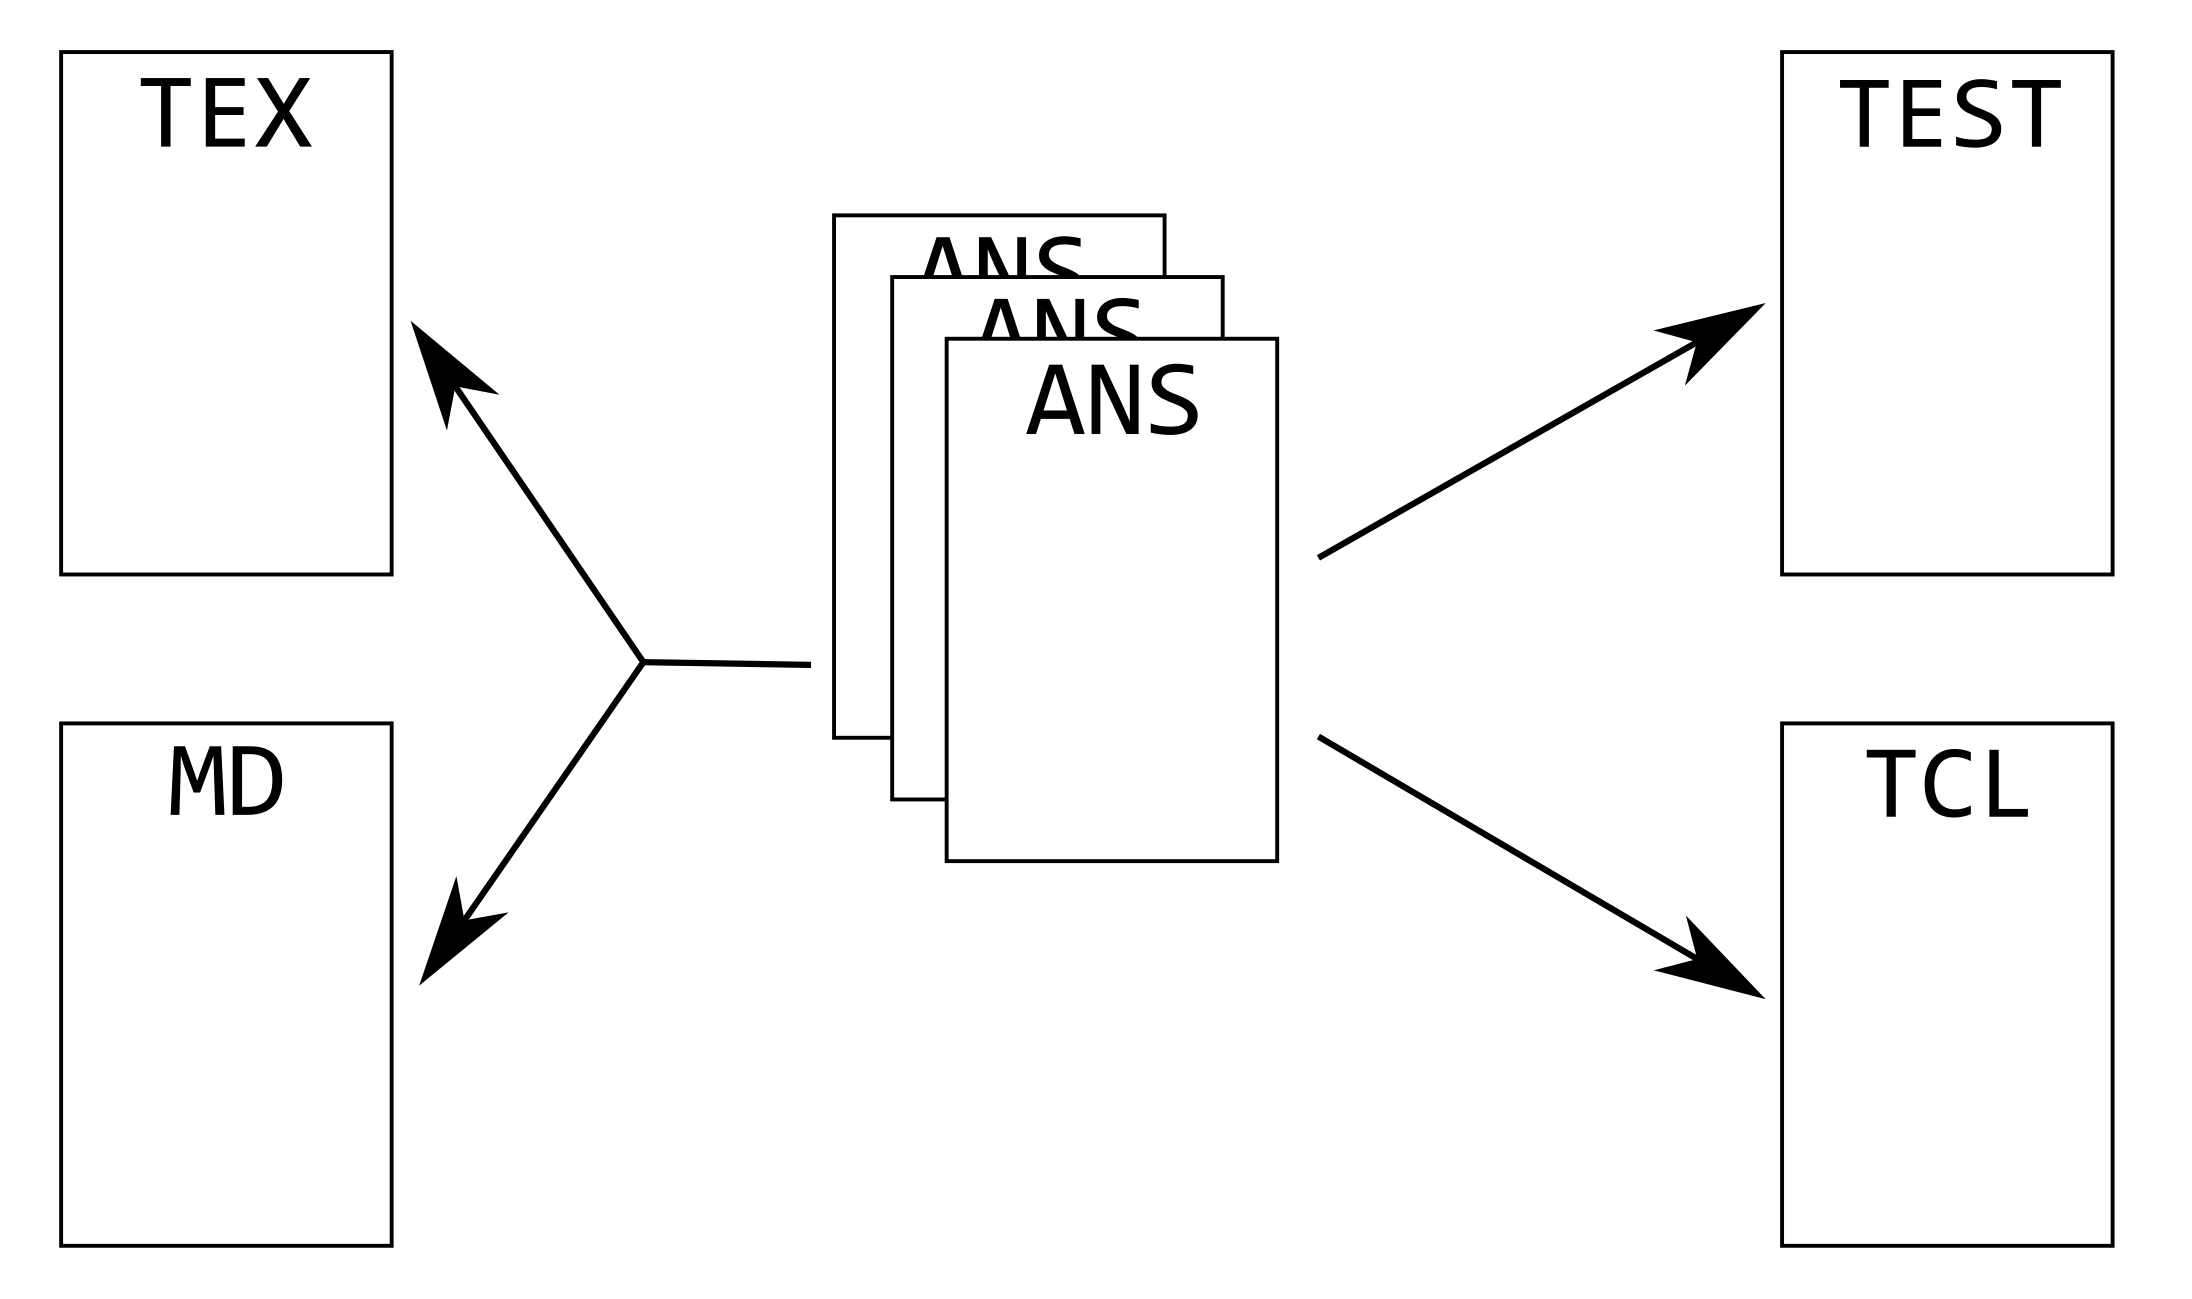
\includegraphics{images/document.png}

In the middle are a bunch of \texttt{.ans} files (ANnotated Source). These are
written with Vim. From the TT tags of those, I extract a \texttt{.test} file.
From the CB tags I extract \texttt{.tcl} source (or Scheme or C source, as the case might
be). From all the tags except TT I extract formatted documentation in Markdown
and \LaTeX{} format. All these extractions are automated using \texttt{make}.
Figures are made with Inkscape.  I create a PDF document from the \LaTeX{}
source using TeXworks. On finishing up ConsTcl, it struck me that the
documentation for this piece of software was fit for a book.

ConsTcl is at least 97\% my own work, but I have ported one part (see page
\pageref{resolving-local-defines}) from ``Scheme 9 from Empty
Space''\footnote{See \texttt{https://t3x.org/s9book/index.html}} by Nils M
Holm\index{Holm, Nils M}, a Lisp interpreter written in C and commented in a similar manner to this
book. Another source of guidance and inspiration was ``Lisp in Small Pieces'' by
Christian Queinnec.

\subsection{About the program listings}
\label{about-the-program-listings}

I have tried to write clear, readable code, but the page format forces me to
shorten lines. I have used two-space indents instead of four-space, a smaller
font, and broken off long lines with a \textbackslash\  at the end of the first
line (a so-called 'tucked-in tail'). Neither of these measures improve
readability, but the alternative is overwriting the margins. Not all broken
lines have the \textbackslash: some are broken inside a
\texttt{\{}\ldots\texttt{\}} block, and some right after a \texttt{^^5b}.

\subsection{About me}
\label{about-me}

I'm a 60 year old former system manager who has been active in programming
since 1979. Currently, since around 25 years, my language of choice is the
rather marginal Tcl\footnote{See \texttt{https://www.tcl-lang.org/}} (it's not
even in the 100 most used languages). Tcl suits me, and there are things that
one can do in Tcl that one can't easily do in other languages. Lisp is a
runner-up in my affections, a language that fascinates me but doesn't fit my
brain very well (though I have written one large piece of software in AutoLisp,
a CAD subsystem for designing drilling boxes).

In addition to my terms as programmer and system manager, I have worked as a
teacher (teaching C/C++ in upper secondary school) and for a short while I
produced textbooks for the department for information technology at
the University of Skövde. I've also been active writing answers at
question-and-answer sites on the web, mainly Stack Overflow.

\subsection{About time}
\label{about-time}

I'd like to thank

\begin{itemize}
\item my children and their lifemates for being awesome.

\item my ex-wife for supporting the printing of the book financially, and, well, for being awesome too.

\item all the wonderful people in my life for being there.
\end{itemize}

And now let's journey into the Interpreter.
